\section{Data mining techniques}
After the completion of the pre-processing, three data mining techniques are applied on the dataset. Each mining technique requires presents its own problems and advantages when used on the chosen dataset. The following section gives a comprehensive account of the the three mining techniques applied. 

\subsection{Association rule mining - Apriori}
Association rule mining is chosen as one of the mining techniques to be used on this dataset because the dataset consists of a lot of categorical data. When the categorical data point is viewed as an "item" in the "transaction" (the degree in a particular college, or row), it gives us a means to identify relationships between the the categorical features. 

A significant portion of the pre-processed dataset also consists of ratio data (census data). To fit this information into the association rule mining, the census data is discretized using equal interval binning. The number of intervals and the width of the intervals are chosen by trial and error. The final results are obtained using 4 bins of the following intervals - (0-20), (20-50), (50-70), (70-100). Further, the entire dataset is now converted into a transaction database format to use for association rule mining. 
Apriori rule is chosen as the association rule mining technique as it provides a quick and easy implementation with good results. A major drawback of the apriori rule is that its multiple scans through the dataset takes makes it inefficient for time. But this is not seen as a major drawback in our implementation as the entire process completes in under a minute on the entire dataset.

To get the frequent itemsets and the association rules using the apriori rule, two parameters have to be tuned to get the desired results. These parameters are minimum\_support(or min\_sup) and minimum\_confidence(or min\_conf). By trial and error min\_sup was chosen to be 15\% and min\_conf was chosen to be 60\%. Min\_sup is chosen to be on the lower side because the dataset is highly dimensional and a lot of "items" do not repeat too many times and hence do not form a part of the association rules. To get more interesting rules, the min\_sup was reduced to a lower range of values.

\begin{table}[htbp]
\caption{Association rules using Apriori}
\label{apriori_res}
\begin{center}
\begin{tabular}{|L|L|c|c|}
\hline
 
\textbf{Antecedent} & \textbf{Consequent}& \textbf{Confidence}& \textbf{Lift} \\
\hline
\{PWD[0-20]$^{\mathrm{a}}$, General[20-50], BC[50-70]\} &  \{Co-education\} & 0.894 & 5.251 \\\hline

\{Postgraduate, Co-education\} & \{Muslim[0-20], PWD[0-20], Other[0-20]\} & 0.893 & 4.818 \\\hline

\{Hostel available, No specialty, Undergraduate, Co-education\} & \{PWD[0-20]\} & 0.998 & 4.909 \\\hline

\{No hostel, BC[70-100], PWD[0-20], Other[0-20]\} & \{No specialty\} & 0.881 & 4.696 \\\hline

\{BC[70-100]\} & \{Undergraduate, Co-education\} & 0.682 & 1.791 \\
\hline
% \multicolumn{4}{l}{$^{\mathrm{a}}$The numbers in square brackets represent the percentage of population in that degree in that college}
\end{tabular}
\end{center}
\end{table}

A few results from the Apriori rule are presented in table~\ref{apriori_res}. The numbers in square brackets represent the percentage of population in that degree in that college. BC stands for Backward Castes, PWD for Public Works Department, and Other represents castes other backward castes. 

The first result shows the distribution of the demographic in co-education colleges with 89.4\% confidence. It is observed that PWD are in very low strength as compared to general caste and Backward castes in co-education colleges which may correlate to the less strength of PWD in higher education colleges in general or the more backward thought process of PWD to only take admission in gender exclusive colleges. 
The second result shows that Muslims, PWD and Other backward castes are not likely to enroll in Postgraduate degrees with 89.3\% confidence. This shows that minority groups stop with undergraduate or lower degrees of education. 
The third result confirms the fact that PWD are very less in number even in co-education undergraduate degrees with hostels. No specialty simply means that the degree is not a specialization which is true for all undergraduate degrees. This rule has a very high confidence of 99.8\%.
The last two rules show that Backward castes (BC) are present in high numbers in undergraduate degrees and this is an encouraging sign for a country like India. This could mean that India's reservation system has worked well and now needs to be reformed to focus more on minorities like muslims, PWD, and other backward castes who show a very low representation even in undergraduate degrees.
The results were filtered using scores like confidence and lift and were chosen manually from a final list of 5000+ generated rules.


\subsection{Clustering}

\begin{figure*}[t]
    \centering
    \subfigure[Assigned cluster labels]{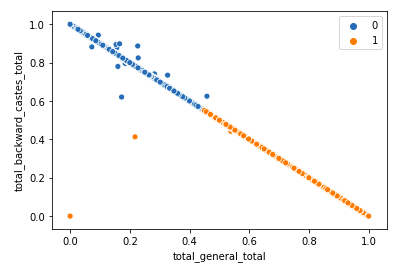
\includegraphics[scale=0.38]{figures/levels1.jpg}}\quad
    \subfigure[Actual labels]{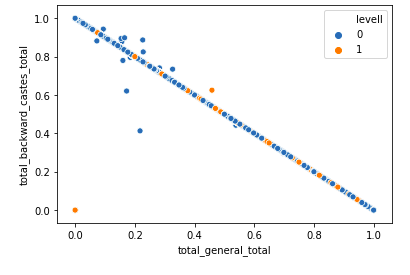
\includegraphics[scale=0.38]{figures/levels2.jpg}}
    \caption{Graphs showing the clustering of different levels of education}
    \label{cluster1_graphs}
\end{figure*}

Given the census-like nature of the dataset, it was decided that clustering could be applied to try and find some interesting results. Upon analyzing the data it is observed that there are 28 numerical attributes, a lot of which are highly sparse, and 10 relevant categorical attributes. 

Cluster analysis can be divided into hierarchical clustering and non-hierarchical clustering techniques. Examples of hierarchical techniques are single linkage, complete linkage, average linkage, median, and Ward. Non-hierarchical techniques include k-means, adaptive k-means, k-medoids, and fuzzy clustering. The goal of K-means clustering is to decrease the summation of square distance among data points and their respective cluster centers. This is an iterative process which eventually converges to output “k” clusters. K-means clustering seemed like the best fit for the dataset because of the census attributes, and the distance between rows would provide information about the differences in population distribution of the rows. Furthermore, some of the categorical attributes have data pertaining to various features like level of education, financing categories for a particular study programme, and exclusivity of females/hostels. These attributes could serve as labels to compare clusters against, after selecting relevant features. In this paper, the traditional K-means clustering algorithm was implemented with Euclidean distance being taken as the distance metric between rows. Reasons for selecting K-means are: simplicity of implementation, speed of convergence and scalability to large datasets such as ours.

Owing to the high dimensionality of the dataset, only a small relevant subset of the numerical attributes are selected for clustering and this relevance is decided by the attribute selected as cluster labels. Upon observing the values for the ``levell'' attribute, it is noticed that the values "Undergraduate" and "Postgraduate" dominated with 326977 and 90643 rows respectively. Thus, k was chosen as two. The attributes "total\_general\_total" and "total\_backward\_castes\_total", the attributes for total general population data and total backward castes data, are chosen for clustering. These attributes are relevant for the aforementioned chosen cluster label attribute, ``levell''. The results obtained are shows in table~\ref{cluster1}. 

At first glance, the precision and recall values look better than expected considering that this was one of the first cluster instances that was performed. However, the plots in Fig~\ref{cluster1_graphs} illustrate the results better. 
It is observed that there is a high precision in the undergraduate sector because it is uniformly spread throughout the dimensions when compared to other degrees and also has a high support count. The high uniformity in the spread is also the reason for the lower recall of the clusters formed here. Whereas, the other degree levels are clustered together near the origin thus when analyzed gives higher recall as all of it can be contained in one cluster but a lower precision as a certain number of undergraduates are also present in the other cluster. Thus clustering does not yield any viable results here.


\begin{table}[htbp]
    \caption{Results of clustering levels of education}
    \label{cluster1}
    \begin{center}
    \begin{tabular}{|c|c|c|c|c|}
    \hline
     
     & \textbf{Precision}& \textbf{Recall}& \textbf{F1 score} & \textbf{Support}  \\
    \hline
    
    label 0$^{\mathrm{a}}$ & 0.79 & 0.69 & 0.74 & 326977 \\\hline
    label 1$^{\mathrm{b}}$ & 0.24 & 0.35 & 0.29 & 90643 \\\hline
    Accuracy &  &  & 0.62 & 417620 \\\hline
    Macro average & 0.52 & 0.52 & 0.51 & 417620 \\\hline
    Weighted average & 0.67 & 0.62 & 0.64 & 417620 \\

    \hline

    \multicolumn{4}{l}{$^{\mathrm{a}}$Undergraduate, $^{\mathrm{b}}$Postgraduate}
    \end{tabular}
    \end{center}
\end{table}

% \begin{figure*}[t]
%     \centering
%     \subfigure[Assigned cluster labels]{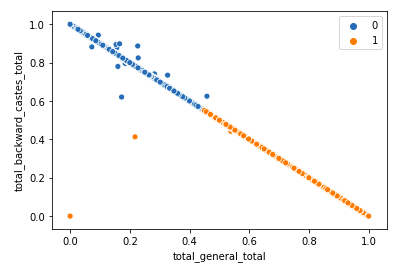
\includegraphics[scale=0.38]{figures/levels1.jpg}}\quad
%     \subfigure[Actual labels]{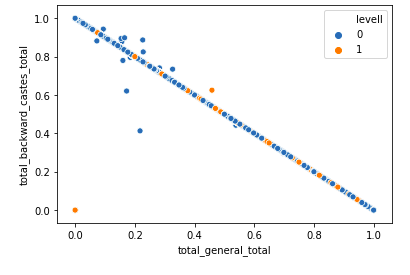
\includegraphics[scale=0.38]{figures/levels2.jpg}}
%     \caption{Graphs showing the clustering of different levels of education}
%     \label{cluster1_graphs}
% \end{figure*}

After considering a few more cluster labels for clustering, like type of college (self financing or not), girl\_exclusive college etc, similar patterns with respect to precision and recall values can be observed, which can be explained by the relevant plots in Fig~\ref{cluster2_graphs}. The results for this clustering are shown in table~\ref{cluster2}.


\begin{figure*}[t]
    \centering
    \subfigure[Assigned cluster labels]{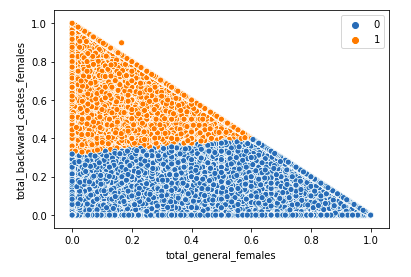
\includegraphics[scale=0.38]{figures/girls2.jpg}}\quad
    \subfigure[Actual labels]{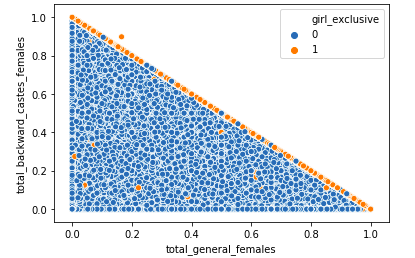
\includegraphics[scale=0.38]{figures/girls1.jpg}}
    \caption{Graphs showing the clustering of gender exclusive colleges}
    \label{cluster2_graphs}
\end{figure*}


\begin{table}[htbp]
    \caption{Results of clustering girls exclusive colleges}
    \label{cluster2}
    \begin{center}
    \begin{tabular}{|c|c|c|c|c|}
    \hline
     
     & \textbf{Precision}& \textbf{Recall}& \textbf{F1 score} & \textbf{Support}  \\
    \hline
    
    label 0$^{\mathrm{a}}$ & 0.93 & 0.75 & 0.83 & 370375 \\\hline
    label 1$^{\mathrm{b}}$ & 0.22 & 0.56 & 0.32 & 47245 \\\hline
    Accuracy &  &  & 0.73 & 417620 \\\hline
    Macro average & 0.58 & 0.66 & 0.58 & 417620 \\\hline
    Weighted average & 0.85 & 0.73 & 0.77 & 417620 \\

    \hline

    \multicolumn{4}{l}{$^{\mathrm{a}}$Not girl exclusive, $^{\mathrm{b}}$Girl exclusive}
    \end{tabular}
    \end{center}
\end{table}

It is thus realized that the cluster label attributes are too skewed towards one of the values for desirable results, and that the available features cannot yield a discernible decision boundary for unsupervised learning techniques such as clustering. 


\subsection{Classification}

The chosen dataset may not seem like a direct fit for a classification task because it is essentially a census dataset. However, classification is attempted on this dataset to find the dependency of all the features of a college degree as a factor in affecting a person's enrollment in that college degree. For example, the task is to find the dependency of features like degree level, number of years of study, location of college, other degree specific features, and also the dependency of the existing demographic of the college on the admission of a minority caste student.

For this classification, the minority caste is chosen to muslims. Hence, the task is to find the dependency of various features on the probability of presence of a muslim in that college degree. There are two output classes which represent if a muslim is likely to be present within that demographic and those types of college degrees. 

The total number of muslims are hence taken as the "Y" and are discretized by using a simple threshold. This threshold is taken as 10\% and depicts that if the population of muslims in a particular college degree are greater than the chosen threshold, it means that they are "present" in that demographic. If their population does not cross this threshold, they are marked as "not present" in that particular college degree.

The required pre-processing techniques were already applied during the general pre-processing step. Features that are relevant for the classification are selected from the pre-processed dataset. The total number of input features are 44. The dataset consists of 375197 examples and these are shuffled and split into train, dev and test sets. Dev and test each consists of 20000 examples and train set contains the rest.

The classification task is carried out using two different learning algorithms - logistic regression and a neural network approach. 

\subsubsection{Logistic regression}
A logistic regression model is trained to predict the presence of a muslim in a particular college degree. Gradient descent is used to optimize the cross entropy loss. L2 regularization is also applied with the regularization parameter $\lambda$ = 10. $\lambda$ is chosen after using a grid search on a logarithmic scale by trying to reduce the variance in the learning (difference between train accuracy and dev accuracy). The accuracies for the logistic regression model are shown in table~\ref{classification_res}.

\begin{table}[htbp]
\caption{Results of classification}
\label{classification_res}   
% \centering
\begin{tabular}{|c|c|c|c|}
\hline
\textbf{} & \textbf{Train accuracy} & \textbf{Dev accuracy} & \textbf{Test accuracy} \\\hline
\textbf{Logistic regression} & 87.42\% & 87.41\% & 87.69\% \\\hline
\textbf{Neural network} & 50.1\% & 12.2\% & 12.4\% \\\hline
\end{tabular} 
\end{table}


\subsubsection{Neural networks}
To try and exceed the performance of the logistic regression model, a neural network is trained to fit the same data. The hyperparameters of the network are chosen by trial and error. Adam is used as the optimizer to optimize the cross entropy loss using a learning rate of 0.0003. The results obtained by training the neural network are far from desirable. The model highly overfits the data as the loss increases with each epoch and the accuracy reduces. Various methods for countering overfitting like regularization at each layer and using dropout layers are implemented but the performance of the model does not increase by a considerable amount. This model is under progress and remains a work that can be implemented in the near future. 

It is observed that logistic regression gives a good enough classifier that can be used to predict whether a student belonging to a certain minority is likely to be present in a given college degree with 87\% accuracy.